%% 美赛模板:正文部分

\documentclass[12pt]{article}  % 官方要求字号不小于 12 号,此处选择 12 号字体

% 本模板不需要填写年份,以当前电脑时间自动生成
% 请在以下的方括号中填写队伍控制号
\usepackage[2307004]{easymcm}  % 载入 EasyMCM 模板文件
\problem{C}  % 请在此处填写题号
\usepackage{mathptmx}  % 这是 Times 字体,中规中矩 
% \usepackage{mathpazo}  % 这是 COMAP 官方杂志采用的更好看的 Palatino 字体,可替代以上的 mathptmx 宏包
% \usepackage{multirow}
\title{Insight from Guessing Words: The Data Exploration and Analysis behind Wordle}  % 标题

% 如需要修改题头(默认为 MCM/ICM),请使用以下命令(此处修改为 MCM)
\renewcommand{\contest}{MCM}

% 文档开始
\begin{document}

% 此处填写摘要内容
\begin{abstract}
    In Wordle, the fun of guessing words and the potential social aspect of the game always attracts many players to the daily challenge. Therefore, it is crucial to increase the traffic to Wordle based on player data and word characteristics.
    
    \textbf{Firstly}, based on an understanding of Wordle's rules and social network features, and by referring to authoritative English morpheme constructions and comprehensive Wordle cheat sheets, we propose heterogeneous spatio-temporal features with word topology-player level and fused social network activity, as well as quantifying the features following data normalization principles. \textbf{After} pre-processing the data, we constructed an \textbf{Autoregressive Integrated Moving Average(ARIMA) Model} to analyze the number of people playing Wordle each day in a time-series manner, and the model performed very well in terms of goodness of fit. In addition to fitting the existing data, further analysis was carried out to derive prediction intervals for future data. We then addressed the question of whether word attributes have an effect on the selection rate of difficult modes by using \textbf{Spearman's Correlation Analysis}, which proved that there was no significant correlation between the two.

    \textbf{Then}, in order to predict the distribution of 1 try-7 or more tries (X), we propose a \textbf{Multiple-input and Multiple-output Extreme Gradient Boosting(MIMO XGBoost) Model} that takes into account their correlation and introduces a percentage sum of 1 constraint in the prediction. Specifically, we trained seven XGBoost regression models temporally synchronously to predict the distribution based on multiple spatio-temporal attributes related to words, i.e. MIMO, and designed a distributed loss function to ensure that the 7 models optimize the parameters towards a common goal. After joint training is completed, each model can be used asynchronously. Experimental results show that our proposed MIMO XGBoost Model brings the frequency closer to 1 than training the XGBoost models independently 7 times, while achieving better accuracy and goodness-of-fit on the test set. We predict the distribution of the number of player attempts for the word EERIE in 2023.3.1 and give the proportional importance of each attribute in difficulty classification, and critically, our MIMO XGBoost Model provides the basis for subsequent classification tasks.

    \textbf{Next}, we defined the average number of attempts (ATN) as a characterization of the difficulty of a particular word for the player and performed a \textbf{Shapiro-Wilk Normality Test} on the ATN, which showed that the ATN was accepted as normally distributed. The ATN was then divided into three intervals according to Empirical Rule, corresponding to the three difficulty levels of easy, normal and hard. The task of classifying word difficulty is then transformed into a prediction task for ATN, which allows us to follow the MIMO XGBoost model described above in predicting the ATN of a given word, while maintaining a high classification accuracy consistent with the prediction task described above. Our classification model shows that EERIE has a hard difficulty.

    \textbf{Finally}, we have collated and analyzed some interesting features of the dataset and provided the patterns from the above analysis and exploration as suggestions to the Puzzle Editor of the New York Times.
    
    \textbf{Keywords}: ARIMA Model, MIMO XGBoost Model, Spearman's Correlation Analysis, Shapiro-Wilk Normality Test.
    % 美赛论文中无需注明关键字。若您一定要使用,
    % 请将以下两行的注释号 '%' 去除,以使其生效
    
    % \textbf{Keywords}: MATLAB, mathematics, LaTeX.

\end{abstract}

\maketitle  % 生成 Summary Sheet
\tableofcontents  % 生成目录


% 正文开始
\section{Introduction}
\subsection{Background}
%The purpose of computation is insight, not numbers. 变为斜体左对齐
\textit{"The purpose of computation is insight, not numbers."} 
% Richard Hamming右对齐
\begin{flushright}
    \textit{-- Richard Hamming}
\end{flushright}



Wordle is one of the most popular word-guessing games in the world. In this game, you can successfully guess the only word of the day in six chances, and share your proud results on social platforms. In a word-guessing game, one of the most curious things is what the word of the day is, and that curiosity and the social nature of the game drive players crazy. But while playing, it's clear that the difficulty of a word can greatly affect the number of attempts a player makes that day, and potentially the traffic of subsequent games, so we hope to find some interesting patterns in our analysis of daily words and make our suggestions to the New York Times Wordle editors.


\subsection{Problem Restatement}
The New York Times asked us to analyze the data provided to us and obtain valuable information, including:
\begin{itemize}
    \item Explain the change in reported results over time and give a forecast for a specific date.
    \item Determine whether the word will affect the percentage of scores reported that were played in Hard Mode.
    \item Predict the distribution of a particular word on a particular day of the reported results
    \item Create a classification model to classify words by difficulty.
    \item Identify the attributes of a given word that are associated with each classification.
    \item Evaluate our model.
    \item Explore the characteristics of the dataset.
\end{itemize}

In order to achieve the above goals, we propose a series of subtasks with precedence constraints. Specifically:
\begin{enumerate}
    \item Make a statistical description of the relevant data, including the central tendency and discrete tendency of the data, and explore the characteristics of the data set.
    \item Analyze the time series diagram of reported results and determine a suitable prediction model by combining the propagation characteristics of social networks.
    \item According to the rules of the Wordle game, extract the features of words and determine the measures of each feature.
    \item Analyzes the correlation between the relevant features of the word and the difficult mode selection rate to determine the influence of the word on the mode chosen by the player.
    \item Aiming at the propagation characteristics of social networks, features are extracted based on dates and their metrics are determined.
    \item Predict the distribution of reported results based on relevant features for dates and words.
    \item Determine a measure of word difficulty based on the rules of the Wordle game and classify the difficulty of words.
\end{enumerate}




\section{Assumptions \& Notations}
\subsection{Assumptions}
We make several assumptions in our model. Later, we may relax these assumptions to optimize our model and make it more applicable to complex real-world environments.
\begin{enumerate}
    \item The records people post on Twitter are accurate.
    \item The data provided does not include incorrect data from competitors or malicious customers.
    \item The number of players recorded per day is equal to the sum of the number of statistics, i.e., there are no omitted or excluded records in any of the provided datasets.
    \item The record uploaded by the player was posted on the day of play.
    \item Each player uploads records at most once a day.
\end{enumerate}


\subsection{Notations}
% \ref{tb:notation}.
% 三线表示例
See in Table \ref{tb:notation}.
\begin{table}[!htbp]
\begin{center}
\caption{Notations}
\begin{tabular}{cl}
	\toprule
	\multicolumn{1}{m{3cm}}{\centering Symbol}
	&\multicolumn{1}{m{8cm}}{\centering Definition}\\
	\midrule
    
	$y_i$&Output value\\
	$\hat{y}_i$&Predicted output value\\
	$W_i$ &Difference value\\
    $PS$ &Weight\\
    $F$ &Word frequency\\
    $ATN$ &Average number of attempts\\
    $L_d$ &Difficulty level\\
    $R_h$ &Percentage in hard mode\\
    $R_{ti}$ &Percentage of i tries\\
    $N_{dw}$ &The number of duplicate words\\
    $N_v$ &The number of vowels\\
    $N_c$ &The number of consonants\\
    $N_{iw}$ &The number of infrequently used words\\
    $N_s$ &The number of syllables\\
    $IF_{rc}$ &Repetition is continuous or not\\
    $IF_{vb}$ &Vowel beginning or not\\
    $IF_{ve}$ &Vowel ending or not\\
    $IF_{vc}$ &Vowel is continuous or not\\
    $IF_{p}$ &Polysemous or not\\
    $IF_{w}$ &Workday or not\\

	\bottomrule
\end{tabular}\label{tb:notation}
\end{center}
\end{table}




\section{Data Preprocessing}
\subsection{Data Cleaning}
By observing the provided data, we found that there are some outliers in the dataset. The Word attribute contains two words with only four letters and one word with six letters, which doesn't follow the rules of the game for guessing five-letter words. There are also numerically anomalous words, for example, in the 1 try-7 tyies attribute, the total percentage of attempts is much greater than 100. Similarly, in the Number of reported results property, the count of two words is well below the average by an order of magnitude. Considering that these words may hurt our modeling, we ignore these anomalous words. 

Finally based on the above process, we summarize the file (word\_ normalization) contains all the words that appeared, and the properties of the words standardization.


\subsection{Feature Extraction \& Quantification}
We only have attributes such as date, word, number of reported results, and distribution of player attempts. In order to predict the distribution of player attempts. we need more attributes to build our model.

According to the rules of Wordle and the characteristics of social networks, we extract the features of data from two dimensions of space and time.

In the spatial dimension, Wordle is an alphabet-oriented English word puzzle game, which determines that the topology of words greatly affects the distribution of the number of attempts by human players. Based on the analysis of Wordle recipes on social networking sites and the morpheme formation of English words, we propose to use the following features (see in Table \ref{tb:notation}) to measure the topology of words:
% 插入图片
\begin{figure}[htbp]
    \centering
    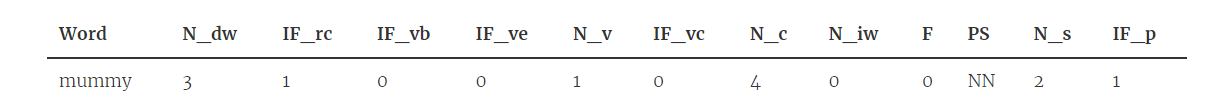
\includegraphics[width=.8\textwidth]{mummy_1.png}
    \caption{Example of the attribute of mummy}\label{fig:mummy_1}
\end{figure}

% \subsubsection{Conclusion of Model 2}
% The results are shown in Figure \ref{fig:result}, where $t$ denotes the time in seconds, and $c$ refers to the concentration of water in the boiler.

% \begin{figure}[htbp]
% \centering
% 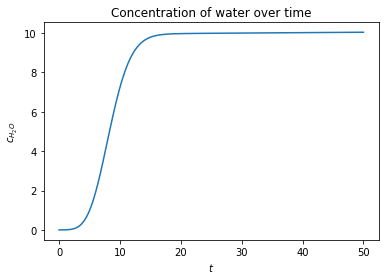
\includegraphics[width=.8\textwidth]{water.png}
% \caption{The result of Model 2}\label{fig:result}
% \end{figure}

% \clearpage
% \subsubsection{Commetary on Model 2}
% The instance of long and wide tables are shown in Table \ref{tb:longtable}.

% % 长表格示例,更多用法请参考 longtable 宏包文档
% % 以下环境及对应参数可实现表格内的自动换行与表格的自动断页
% % 您也可以选择自行载入 tabularx 宏包,并通过 X 参数指定对应列自动换行
% \begin{longtable}{ p{4em} p{14em} p{14em} }
% \caption{Basic Information about Three Main Continents (scratched from Wikipedia)}
% \label{tb:longtable}\\
% \toprule
% Continent & Description & Information \\
% \midrule
% Africa & Africa Continent is surrounded by the Mediterranean Sea to the
% north, the Isthmus of Suez and the Red Sea to the northeast, the Indian
% Ocean to the southeast and the Atlantic Ocean to the west. &
% At about 30.3 million km$^2$ including adjacent islands, it covers 6\%
% of Earth's total surface area and 20\% of its land area. With 1.3
% billion people as of 2018, it accounts for about 16\% of the world's
% human population. \\
% \midrule
% Asia & Asia is Earth's largest and most populous continent which
% located primarily in the Eastern and Northern Hemispheres.
% It shares the continental landmass of Eurasia with the continent
% of Europe and the continental landmass of Afro-Eurasia with both
% Europe and Africa. &
% Asia covers an area of 44,579,000 square kilometres, about 30\%
% of Earth's total land area and 8.7\% of the Earth's total surface
% area. Its 4.5 billion people (as of June 2019) constitute roughly
% 60\% of the world's population. \\
% \midrule
% Europe & Europe is a continent located entirely in the Northern
% Hemisphere and mostly in the Eastern Hemisphere. It comprises the
% westernmost part of Eurasia and is bordered by the Arctic Ocean to
% the north, the Atlantic Ocean to the west, the Mediterranean Sea to
% the south, and Asia to the east. &
% Europe covers about 10,180,000 km$^2$, or 2\% of the Earth's surface
% (6.8\% of land area), making it the second smallest
% continent. Europe had a total population of about 741 million (about
% 11\% of the world population) as of 2018. \\
% \bottomrule
% \end{longtable}

% Figure \ref{fig:subfigures} gives an example of subfigures. Figure \ref{subfig:left} is on the left, and Figure \ref{subfig:right} is on the right.

% % 子图(多图并列)示例,更多用法请参考 subfigure 宏包文档
% % 如果您只希望几张图并列,不需要额外的 caption,那么在 figure 环境中
% % 连续插入总宽度不超过 \textwidth 的多个 \includegraphics 命令即可
% \begin{figure}[htbp]
% \centering
% \begin{subfigure}[b]{.4\textwidth}
% 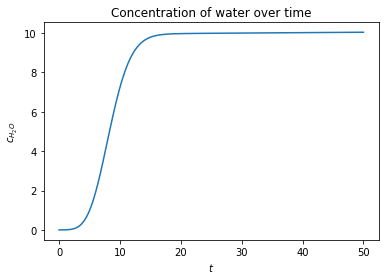
\includegraphics[width=\textwidth]{water.png}
% \caption{Image on the left}\label{subfig:left}
% \end{subfigure}
% \begin{subfigure}[b]{.4\textwidth}
% 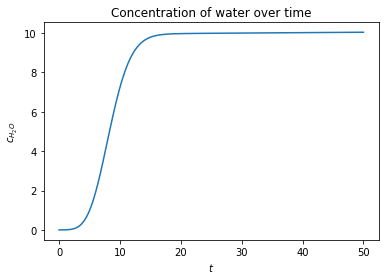
\includegraphics[width=\textwidth]{water.png}
% \caption{Image on the right}\label{subfig:right}
% \end{subfigure}
% \caption{Two images}\label{fig:subfigures}
% \end{figure}


\subsection{Data Standardization}
Standardization is a necessary step. Here we use the Min-Max Normalization method, which uses raw data based on its maximum value, Max, and minimum value, Min. The processed data fit the interval distribution from 0 to 1. The conversion function is:
\begin{equation}\label{eq:normal}
    \frac{x-x_{\min }}{x_{\max }-x_{\min }}
\end{equation}

After the standardization step, the standard data of uniform interval is obtained.
\begin{figure}[htbp]
    \centering
    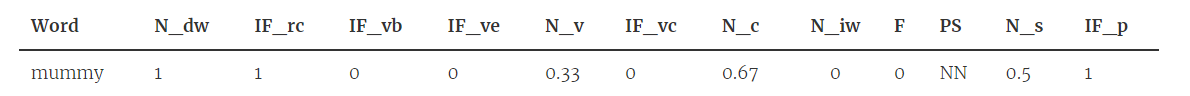
\includegraphics[width=.8\textwidth]{mummy_2.png}
    \caption{Example of the attribute of mummy after standardization}\label{fig:mummy_2}
\end{figure}


\subsection{Modeling Framework}
Our modeling framework can be illustrated as shown in Figure \ref{fig:framework}.
\begin{figure}[htbp]
    \centering
    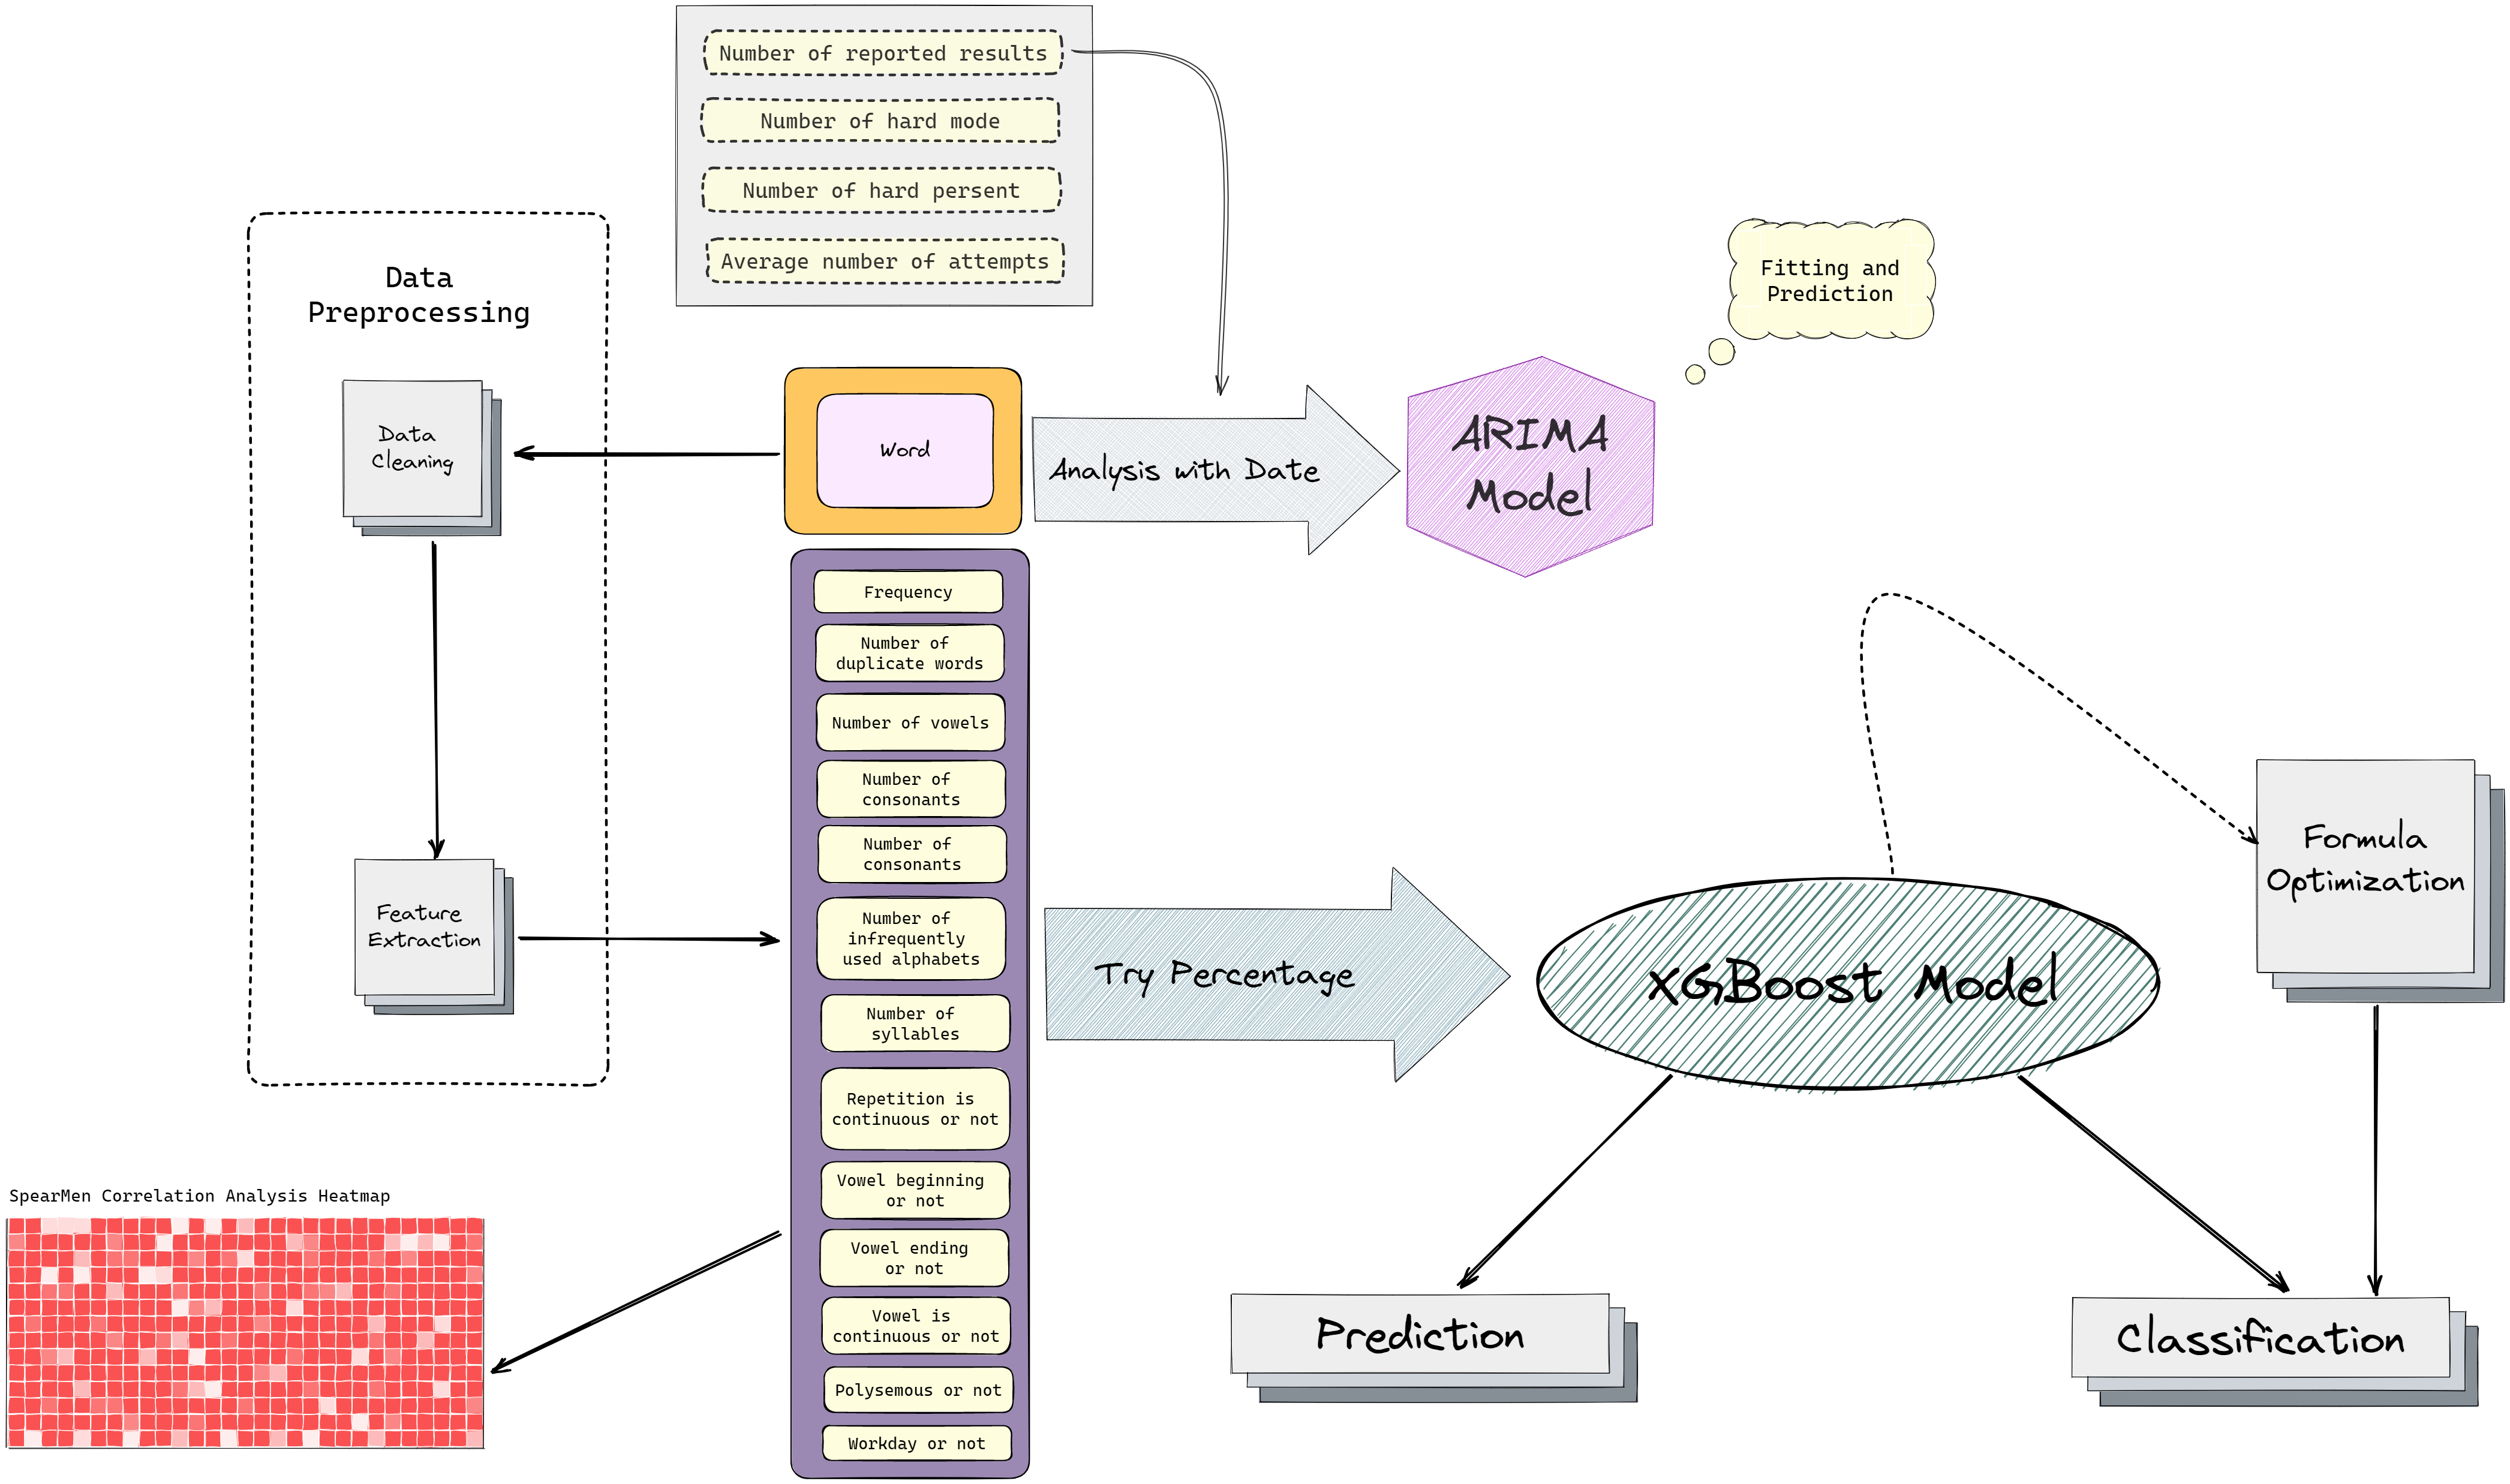
\includegraphics[width=.8\textwidth]{framework.png}
    \caption{Modeling framework}\label{fig:framework}
\end{figure}

\section{ARIMA Model}
In this section, we use the Autoregressive Integrated Moving Average(ARIMA) prediction model as a data simulation measure for the future online number of Wordle. Based on the number performance of Wordle in historical time, At the same time, the lagged moving average is used to obtain a smooth time series, so as to make a rough estimate of the number of people online at a certain time in the future. We then performed feature extraction on the word attributes, using the similarity matrix to analyze whether any attribute of the word affects the percentage of the total number of people participating in the difficult pattern.


\subsection{Model Review}
\subsubsection{Auto Regression(AR) Model}
The autoregressive model describes the relationship between the current value and the historical value and uses the historical time data of the variable to predict itself.

In general, the formula of the P-order autoregressive process is defined as follows:
\begin{equation}\label{eq:AR_1}
    y_{t}=\mu+\sum_{i=1}^{p} \gamma_{i} y_{t-i}+\epsilon_{t}
\end{equation}

General P-order autoregressive model AR:
\begin{equation}\label{eq:AR_2}
    x_{t}=\alpha_{1} X_{t-1}+\alpha_{2} X_{t-2}+\ldots+a_{p} x_{t-p}+μ_{t}
\end{equation}

As can be seen from the formula, the current value is predicted by the historical value, and p is an order in the autoregressive model, which indicates that the historical value of several epochs is used to predict the current value.


\subsubsection{Moving Average(MA) Model}
Moving averages focus on the accumulation of error terms in autoregressive models.

Among them, the formula of the q-order self-MA model is defined as follows:
\begin{equation}\label{eq:MR_1}
    y_{t}=\mu+\epsilon_{t}+\sum_{i=1}^{q} \theta_{i} \epsilon_{t-i}
\end{equation}

In the AR model, if it is not white noise, it is usually considered to be a moving average of order q:
\begin{equation}\label{eq:MR_2}
u_{t}=\varepsilon_{t}+\beta_{1} \varepsilon_{t-1}+\ldots+\beta_{q} \varepsilon_{t-q}
\end{equation}

The moving average method can effectively eliminate random fluctuations in the forecast.


\subsubsection{Autoregressive Moving Average (ARMA) Model}
The autoregressive moving average model consists of two parts: the autoregressive part and the moving average part. The regression equation is expressed as follows:
\begin{equation}\label{eq:ARMA}
    y_{t}=\mu+\sum_{i=1}^{p} \gamma_{i} y_{t-i}+\epsilon_{t}+\sum_{i=1}^{q} \theta_{i} \epsilon_{t-i}
\end{equation}

It can be seen from the regression equation that the autoregressive moving average model combines the advantages of AR and MA. In the ARMA model, the autoregressive process is responsible for quantifying the relationship between the current data and the previous data, and the moving average process is responsible for solving the problem of random changes.


\subsubsection{Differential Autoregressive Moving Average (ARIMA) Model}
The Autoregressive model (AR), the moving average model (MA), and the difference method (I) are combined to obtain the differential autoregressive moving average model ARIMA (p, d, q), where d is the order of the difference to be performed on the data, and ARIMA is the ARMA model after the difference.


\subsection{Model Analysis}
Step size selection:

Considering that the ARIMA model has high uncertainty for the result of too long prediction, we add a sliding window to explore the number of future players, and the step size is set to 7 so that the time unit of prediction is changed from days to weeks, which can greatly reduce the number of predictions.
\begin{figure}[htbp]
\centering
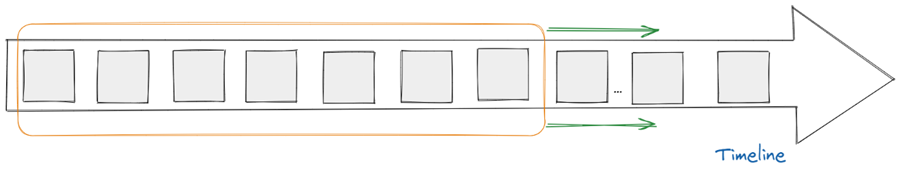
\includegraphics[width=.7\textwidth]{img/timeStep.png}
\caption{Slider window model with step size 7}\label{fig:result}
\end{figure}

ARIMA model requires that sequences meet stationarity. Check the results of the ADF test, and analyze whether it can significantly reject the hypothesis of sequence instability according to the analysis t value (P<0.05).
%Table
% Please add the following required packages to your document preamble:

\begin{table}[]
\centering
\begin{tabular}{|clclcccccc|}
\hline
\multicolumn{10}{|c|}{ADF test table} \\ \hline
\multicolumn{2}{|c|}{\multirow{3}{*}{variables}} &
  \multicolumn{2}{c|}{\multirow{3}{*}{Order of difference}} &
  \multicolumn{1}{c|}{\multirow{3}{*}{t}} &
  \multicolumn{1}{c|}{\multirow{3}{*}{P}} &
  \multicolumn{1}{c|}{\multirow{3}{*}{AIC}} &
  \multicolumn{3}{c|}{Critical value} \\ \cline{8-10} 
\multicolumn{2}{|c|}{} &
  \multicolumn{2}{c|}{} &
  \multicolumn{1}{c|}{} &
  \multicolumn{1}{c|}{} &
  \multicolumn{1}{c|}{} &
  \multicolumn{1}{c|}{\multirow{2}{*}{1\%}} &
  \multicolumn{1}{c|}{\multirow{2}{*}{5\%}} &
  \multicolumn{1}{l|}{\multirow{2}{*}{10\%}} \\
\multicolumn{2}{|c|}{} &
  \multicolumn{2}{c|}{} &
  \multicolumn{1}{c|}{} &
  \multicolumn{1}{c|}{} &
  \multicolumn{1}{c|}{} &
  \multicolumn{1}{c|}{} &
  \multicolumn{1}{c|}{} &
  \multicolumn{1}{l|}{} \\ \hline
\multicolumn{2}{|c|}{\multirow{3}{*}{Average   Number}} &
  \multicolumn{2}{c|}{0} &
  \multicolumn{1}{c|}{-3.276} &
  \multicolumn{1}{c|}{0.016**} &
  \multicolumn{1}{c|}{651.242} &
  \multicolumn{1}{c|}{-3.616} &
  \multicolumn{1}{c|}{-2.941} &
  -2.609 \\ \cline{3-10} 
\multicolumn{2}{|c|}{} &
  \multicolumn{2}{c|}{1} &
  \multicolumn{1}{c|}{-4.002} &
  \multicolumn{1}{c|}{0.001***} &
  \multicolumn{1}{c|}{627.622} &
  \multicolumn{1}{c|}{-3.616} &
  \multicolumn{1}{c|}{-2.941} &
  -2.609 \\ \cline{3-10} 
\multicolumn{2}{|c|}{} &
  \multicolumn{2}{c|}{2} &
  \multicolumn{1}{c|}{-3.867} &
  \multicolumn{1}{c|}{0.002***} &
  \multicolumn{1}{c|}{620.775} &
  \multicolumn{1}{c|}{-3.621} &
  \multicolumn{1}{c|}{-2.944} &
  -2.61 \\ \hline
\end{tabular}
\caption{Note: ***, **, * represent significance levels of 1\%, 5\%, and 10\% respectively}
\end{table}



By looking up the table and comparing the difference sequence images, we conclude that the best difference value is order 1. When the difference is order 1, the significance P value is 0.001***, showing significance on the level, rejecting the null hypothesis, and the series is a stationary time series.

\begin{figure}[htbp]
\centering
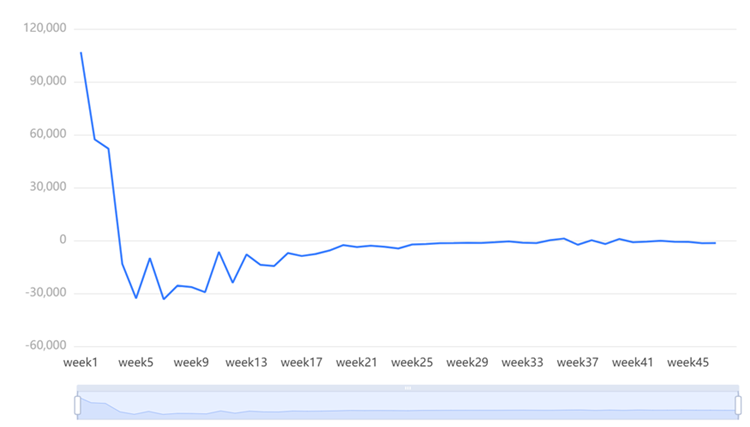
\includegraphics[width=.5\textwidth]{img/difference.png}
\caption{Optimal difference map}\label{fig:result}
\end{figure}

Check the comparison chart of the data before and after differences to determine whether it is stable. At the same time, the time series is biased (autocorrelation analysis), and its p and q values are estimated according to the censoring situation, as shown in the following figure:

\begin{figure}[htbp]
\centering
\begin{subfigure}{.4\textwidth}
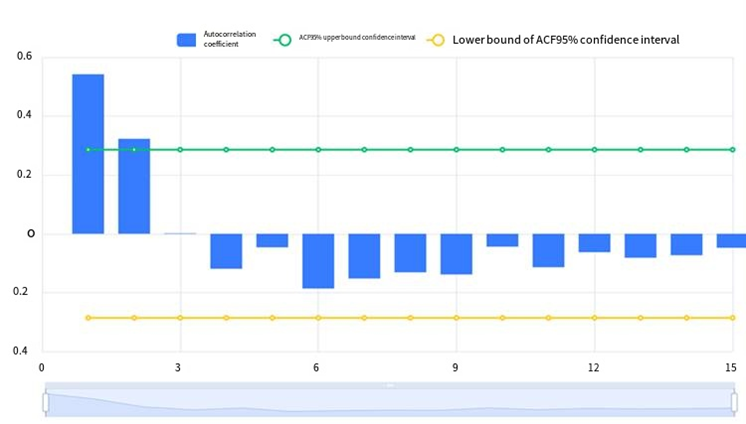
\includegraphics[width=\textwidth]{img/ACF.png}
\caption{Final differential data autocorrelogram (ACF)}
\end{subfigure}
\begin{subfigure}{.4\textwidth}
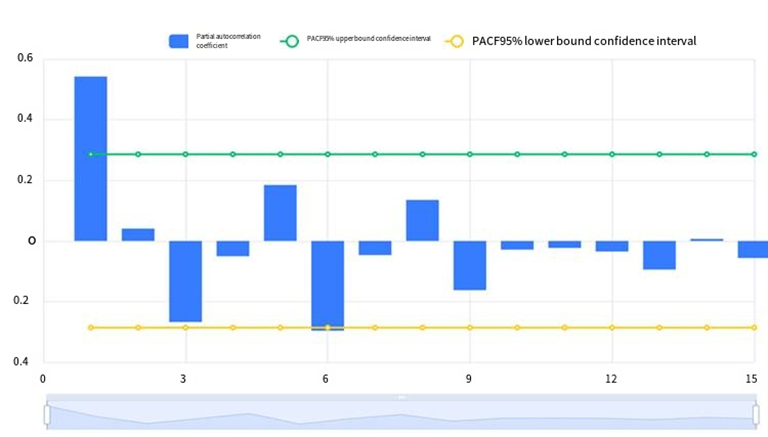
\includegraphics[width=\textwidth]{img/PCAF.png}
\caption{Final differential data Partial Autocorrelation Map (PACF)}
\end{subfigure}
\caption{}
\end{figure}
We finally determined the ARIMA model as ARIMA(2,1,0). The model parameter table is as follows. The table shows the results of this model test, including the sample number, degrees of freedom, Q statistics, and the goodness of fit of the information criterion model.

% Table
% \usepackage{multirow}
\begin{table}[]
\centering
\begin{tabular}{|ccc|}
\hline
\multicolumn{3}{|c|}{ARIMA   model (1,1,0) Test Table}                                          \\ \hline
\multicolumn{1}{|c|}{Item}              & \multicolumn{1}{c|}{Symbol}         & Value           \\ \hline
\multicolumn{1}{|c|}{}                  & \multicolumn{1}{c|}{Df   Residuals} & 45              \\ \hline
\multicolumn{1}{|c|}{Number of samples} & \multicolumn{1}{c|}{N}              & 48              \\ \hline
\multicolumn{1}{|c|}{\multirow{5}{*}{Q statistic}}           & \multicolumn{1}{c|}{Q6(P   value)} & 3.317(0.069*) \\ \cline{2-3} 
\multicolumn{1}{|c|}{}                  & \multicolumn{1}{c|}{Q12(P value)}   & 13.838(0.031**) \\ \cline{2-3} 
\multicolumn{1}{|c|}{}                  & \multicolumn{1}{c|}{Q18(P value)}   & 18.141(0.111)   \\ \cline{2-3} 
\multicolumn{1}{|c|}{}                  & \multicolumn{1}{c|}{Q24(P value)}   & 18.315(0.435)   \\ \cline{2-3} 
\multicolumn{1}{|c|}{}                  & \multicolumn{1}{c|}{Q30(P value)}   & 18.384(0.784)   \\ \hline
\multicolumn{1}{|c|}{\multirow{2}{*}{Information criterion}} & \multicolumn{1}{c|}{AIC}           & 1041.317      \\ \cline{2-3} 
\multicolumn{1}{|c|}{}                  & \multicolumn{1}{c|}{BIC}            & 1046.867        \\ \hline
\multicolumn{1}{|c|}{Goodness of fit}   & \multicolumn{1}{c|}{R²}             & 0.977           \\ \hline
\end{tabular}
\caption{Note: ***, **, * represent significance levels of 1\%, 5\%, and 10\% respectively}
\end{table}



Finally, we obtain the time series plot and prediction interval plot for the simulated average number of people, as shown in the following figure:

\begin{figure}[htbp]
\centering
\begin{subfigure}{.4\textwidth}
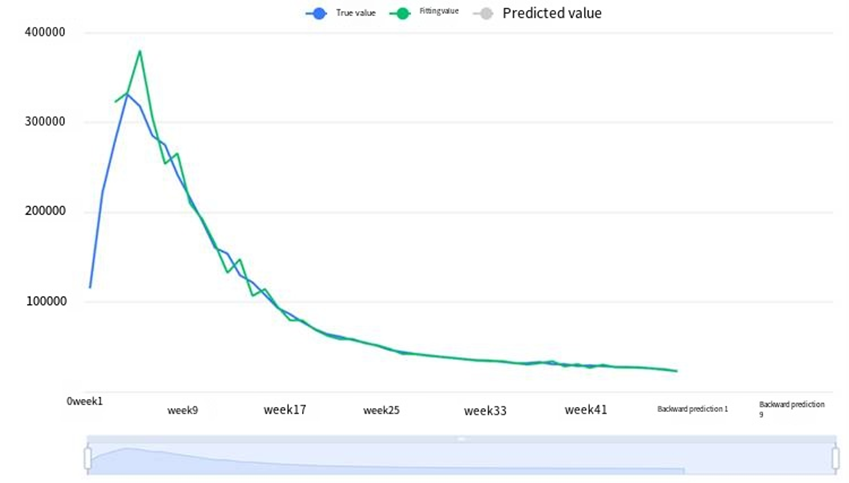
\includegraphics[width=\textwidth]{img/TSP.png}
\caption{Time series graph of average population}\label{subfig:left}
\end{subfigure}
\begin{subfigure}{.4\textwidth}
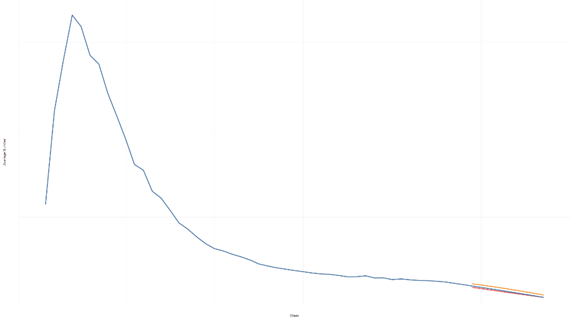
\includegraphics[width=\textwidth]{img/end .png}
\caption{The forecast range of the average population}\label{subfig:right}
\end{subfigure}
\caption{}
\end{figure}

The prediction interval is obtained by predicting the minimum number of players and the maximum number of players per week and taking their numbers as the left and right critical values of the interval to obtain a more reliable value. 


\subsection{The Similarity Matrix}
Conjecture: Since in the Wordle game, the player cannot know which word is until the end of the game, this should not affect the player's choice of a difficult mode. Based on this conjecture, we carry out the following analysis.

In analyzing the correlation between word attributes and the percentage of people who participated in difficulties, we chose to use Spearman correlation analysis. Pearson correlation analysis is mainly used to analyze the relationship between two quantitative variables that meet normal distribution. If the two variables include rank variables, or the variables do not meet normal distribution, or the distribution type of the variables is unknown, Spearman correlation analysis is a more appropriate analysis method. The basic idea of Spearman correlation analysis is: rank transformation is performed on two variables X and Y respectively, denoted by rank order RX and RY, and the average rank is taken as the rank of each data. The calculation formula of Spearman correlation coefficient $r$ is:
\begin{equation}\label{eq:spearman}
    r_{s}=\frac{\sum\left(R_{X}-\overline{R_{X}}\right)\left(R_{Y}-R_{Y}\right)}{\sqrt{\sum\left(R_{X}-\overline{R_{X}}\right)^{2} \sum\left(R_{Y}-\overline{R_{Y}}\right)^{2}}}=\frac{\sum R_{X} R_{Y}-\frac{\left(\sum R_{X}\right)\left(\sum R_{Y}\right)}{n}}{\sqrt{\left(\sum R_{X}^{2}-\frac{\left(\sum R_{X}\right)^{2}}{n}\right)\left(\sum R_{Y}^{2}-\frac{\left(\sum R_{Y}\right)^{2}}{n}\right)}}
\end{equation}

\begin{figure}[htbp]
    \centering
    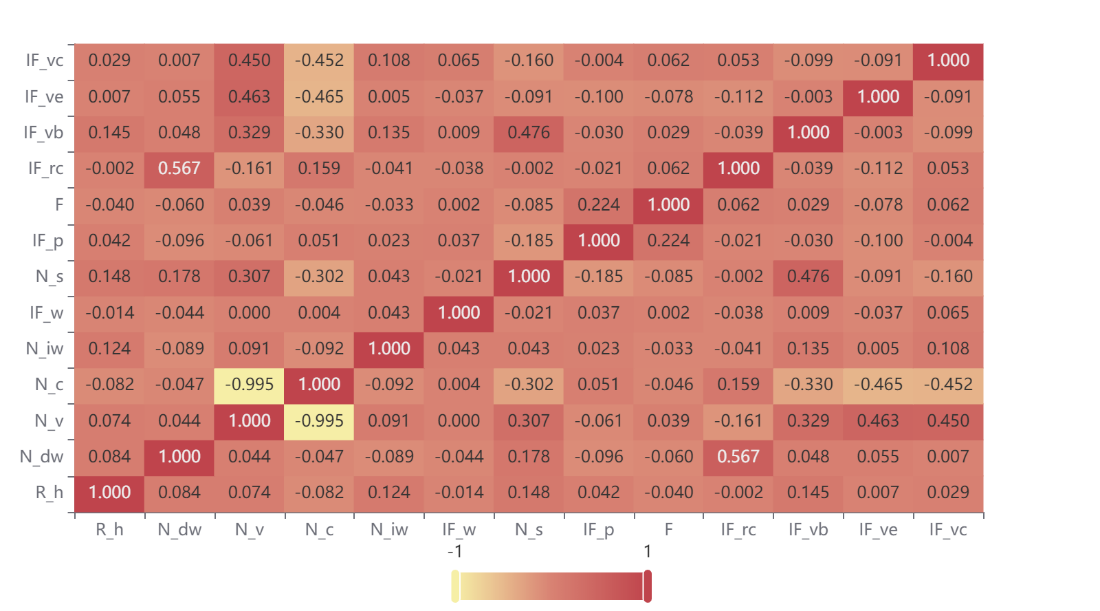
\includegraphics[width=.8\textwidth]{sim_matrix.png}
    \caption{Similarity matrix}\label{fig:sim_matrix}
\end{figure}

It can be clearly seen from the figure that there is a very weak correlation and the irrelevant relationship between the percentage of people who participate in difficult mode and the attributes of words, so it can be concluded that the attributes of words do not affect the number of people who choose to participate in difficult mode on the day of the game.




%        Q2全部
\section{MIMO XGBoost Model}
The model should not only use the feature values extracted in Section 3.1 but also the time dimension is an important influencing factor. We summarize the $IF_w$ attribute according to the change in the activity of the social network over time. In summary, we optimize the XGBoost regression prediction model and based on the conclusion of Section 3.1, we take the attributes of words and time attributes as input values, predict the distribution of (1,2,3,4,5,6, X), and quantitatively test the accuracy of the model.
\subsection{XGBoost Model Analysis}
\subsubsection{Decision Tree Ensembles}
A tree ensemble model consists of a set of classification and regression trees (CART), mathematically speaking, we can write the model in the following form:
\begin{equation}
\hat{y}_i = \sum_{k=1}^K f_k(x_i), f_k \in \mathcal{F}
\end{equation}

Where K is the number of trees,f is the space of functions of F, and F is the set of CART possibilities. The objective function of the above model is given by the following equation:
\begin{equation}
\text{obj}(\theta) = \sum_i^n l(y_i, \hat{y}_i) + \sum_{k=1}^K \omega(f_k)
\end{equation}

Where the first term is the loss function, and the second term is the regularization parameter.
\subsubsection{Tree Boosting}
For the current tree model, the learning method is to define the objective function and optimize it. We have defined the objective function above.
\begin{equation}
\text{obj}(\theta) = \sum_i^n l(y_i, \hat{y}_i) + \sum_{k=1}^K \omega(f_k)
\end{equation}

Considering the difficulty of learning the tree structure, we also adopt the addition strategy to optimize it, adding a new tree each time:

\begin{equation}
\begin{split}\hat{y}_i^{(0)} &= 0\\
\hat{y}_i^{(1)} &= f_1(x_i) = \hat{y}_i^{(0)} + f_1(x_i)\\
\hat{y}_i^{(2)} &= f_1(x_i) + f_2(x_i)= \hat{y}_i^{(1)} + f_2(x_i)\\
&\dots\\
\hat{y}_i^{(t)} &= \sum_{k=1}^t f_k(x_i)= \hat{y}_i^{(t-1)} + f_t(x_i)\end{split}
\end{equation}

Then select the tree that can optimize the objective function, and consider using the mean square error (MSE) as the loss function:

\begin{equation}\label{eq:origin}
\begin{split}\text{obj}^{(t)} & = \sum_{i=1}^n (y_i - (\hat{y}_i^{(t-1)} + f_t(x_i)))^2 + \sum_{i=1}^t\omega(f_i) \\
          & = \sum_{i=1}^n [2(\hat{y}_i^{(t-1)} - y_i)f_t(x_i) + f_t(x_i)^2] + \omega(f_t) + \mathrm{constant}\end{split}
\end{equation}

The loss function is obtained by Taylor expansion to second order and removing all constants:
\begin{equation}
\sum_{i=1}^n [g_i f_t(x_i) + \frac{1}{2} h_i f_t^2(x_i)] + \omega(f_t)
\end{equation}

Under this definition, the value of the objective function is determined only by $g_i$ and ℎ $h_i$. This is how XGBoost supports custom loss functions.

\subsubsection{The Structure Score}
After reformulating the tree model, we can write the target value as:

\begin{equation}
\begin{split}\text{obj}^{(t)} &\approx \sum_{i=1}^n [g_i w_{q(x_i)} + \frac{1}{2} h_i w_{q(x_i)}^2] + \gamma T + \frac{1}{2}\lambda \sum_{j=1}^T w_j^2\\
&= \sum^T_{j=1} [(\sum_{i\in I_j} g_i) w_j + \frac{1}{2} (\sum_{i\in I_j} h_i + \lambda) w_j^2 ] + \gamma T\end{split}
\end{equation}

If the structure part q of the tree is known, the objective function can be used to find the optimal Wj and obtain the optimal objective function value. Its essence can be reduced to the problem of solving the minimum value of quadratic function. The solution is:
\begin{equation}
\begin{split}w_j^\ast &= -\frac{G_j}{H_j+\lambda}\\
\text{obj}^\ast &= -\frac{1}{2} \sum_{j=1}^T \frac{G_j^2}{H_j+\lambda} + \gamma T\end{split}
\end{equation}

\subsection{Model Optimization}
\subsubsection{Deficiency of XGBoost regression prediction model}
The XGBoost model we are using here is a multi-input single-output model that can only predict one/at a time. If only this model is used, the different/are not correlated and may result in the total percentage sum of the forecast being much greater than or less than 100, with the subscript of the word black:
\begin{figure}[htbp]
\centering
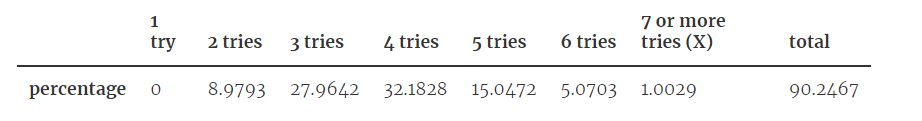
\includegraphics[width=.8\textwidth]{111.png}
\caption{Application of XGBoost to the word black}\label{fig:result}
\end{figure}

Using a simple XGBoost regression forecasting model to forecast the world, find the sum of forecast from 100, the deflection, in other words, $R_{ti}$ lack of correlation between.

\subsubsection{Optimize the XGBoost model}
In practice, the relationship between $R_{ti}$ is as follows:
\begin{equation}
total=\hat{y}_1+\hat{y}_2+...+\hat{y}_7={\textstyle \sum_{1}^{7}} \hat{y}_i=100
\end{equation}

Because of rounding, the error value of the final data is allowed to be 1.
This, in turn, can calculate the difference between the predicted values and 100 value $V_d$, computation formula is as follows:

\begin{equation}
V_d=100-total=100-{\textstyle \sum_{1}^{7}} \hat{y}_i
\end{equation}

For this model, each predicted value has an impact on $V_d$, and their respective weights are $w_i$:
\begin{equation}
W_i=\hat{y}_i\times10^{-2}
\end{equation}

Based on the weight of the predicted value and difference value, the influence value of each predicted value on the deviation value ($V_{di}$) is given. The relevant formula is as follows:
\begin{equation}\label{eq:difference}
V_{di}=W_i\times V_d=\hat{y}_i\times10^{-2}\times(100-{\textstyle \sum_{1}^{7}} \hat{y}_i)
\end{equation}

Formula \ref{eq:difference} is added into the objective function of the XGBoost regression model (Formula \ref{eq:origin}) as a supplement to the cost function, then the optimized XGBoost regression model can be obtained, and the optimized model can conform to the correlation between each $R_{ti}$, the formula is as follows:

\begin{equation}
\begin{split}
\text{obj}(\theta) &= \sum_i^n l(y_i, \hat{y}_i)^{'} + \sum_{i=1}^t \omega(f_k)
\\
&= \sum_{i=1}^n [y_i - (\hat{y}_i^{(t-1)} + f_t(x_i))^2+V_{di}^2] + \sum_{i=1}^t\omega(f_i) \\
&=\sum_{i=1}^n [2(\hat{y}_i^{(t-1)} - y_i)f_t(x_i) + f_t(x_i)^2+(\hat{y}_i\times10^{-2}\times(1-{\textstyle \sum_{1}^{7}} \hat{y}_i))^2] + \omega(f_t) + \mathrm{constant}
\end{split}
\end{equation}

Taking the Taylor expansion of the loss function to second order and removing all the constants yields:
\begin{equation}
\sum_{i=1}^n [g_i f_t(x_i) + \frac{1}{2} h_i f_t^2(x_i)] + \omega(f_t)
\end{equation}

The value of the objective function only depends on $g_i$ and $h_i$. In line with the way XGBoost supports custom loss functions.
\subsection{Model Evaluation}\label{evaluation}
\subsubsection{Model Measurement}
Using 70\% of the data in the 'word normalization' file as the training set and the rest as the test set, the Percentage of the i tries in the test set is calculated, and the predicted value of each tries is obtained. In Table i, the left side is the predicted value, and the right side is the real value.

\begin{figure}[htbp]
\centering
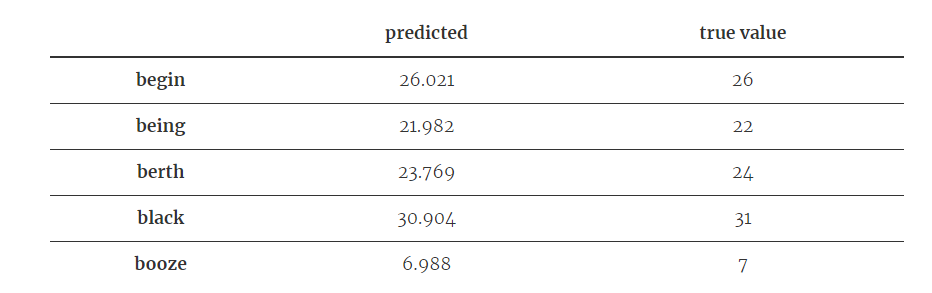
\includegraphics[width=.8\textwidth]{img/image.png}
\caption{3 tries Partial table of test samples versus real samples}\label{fig:result}
\end{figure}

From the above table, we can see that all the predicted results and the true results are very different, only 0.24 difference at most.

\subsubsection{Quantitative Evaluation}
We use several common statistical parameters to quantitatively test the conclusions obtained from the data. Root Mean Square Error () is the first measure we choose to use, which can effectively test the accuracy of the predicted value. The related formula is as follows:

\begin{equation}\label{eq:RMSE}
R M S E=\sqrt{\frac{1}{n} \sum_{i=1}^{n}\left(\hat{y}_{i}-y_{i}\right)^{2}}
\end{equation}

In addition, we choose the Mean Absolute Error (MAE) as the accuracy measure. MAE can reflect the actual situation of the predicted value error, and the relevant formula is as follows:

\begin{equation}\label{eq:MAE}
\mathrm{MAE}=\frac{1}{\mathrm{n}} \sum_{\mathrm{i}=1}^{\mathrm{n}}\left|\hat{\mathrm{y}}_{\mathrm{i}}-\mathrm{y}_{\mathrm{i}}\right|
\end{equation}

Finally, the conventional goodness-of-fit $R^2$ is selected as the overall evaluation of model fitting. The following table shows the test result statistics of the test set and the training set:

\begin{figure}[htbp]
\centering
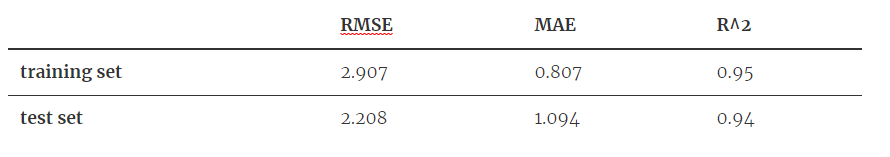
\includegraphics[width=.8\textwidth]{img/compare.png}
\caption{Evaluation results of EERIE}\label{fig:result}
\end{figure}

The evaluation indexes of the training set were $RMSE=2.907$ , $MAE=0.807$,$R^2=0.95$It can be considered that our optimized model has a good fit.
The evaluation indexes of the test set are RMSE=2.208, MAE=1.094, and the goodness of fit indicates that the prediction of the model is very accurate.

\subsubsection{Predicting the Outcome of EERIE}
Using the model above, we produce a prediction for EERIE on March 1, 2023 (the result for total may not match 100\% due to rounding).

\begin{figure}[htbp]
\centering
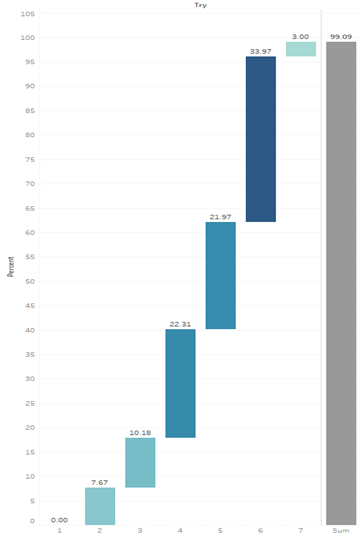
\includegraphics[width=.3\textwidth]{img/predict.png}
\caption{Plot of the prediction results for EERIE}\label{fig:predict}
\end{figure}

Based on the evaluation conclusions of Section 3.2, we have strong confidence in the prediction of the distribution of EERIE words $R_{ti}$.

\subsubsection{ Uncertainty}
Although our prediction model has a good degree of fit and prediction accuracy, it is a theoretical model trained based on the assumptions in Section 2.1. The real situation is more complex, and there are many uncontrollable factors that may impact our prediction results. For example, the act of Posting grades on Twitter is highly subjective. If the word EERIE is too complicated for many people, it may reduce people's grades, and bad grades may cause them not to upload their grades on Twitter. But if we ignore this subjective impact, I have strong confidence in our predictive model in the theoretical case.



\section{Empirical Rule Based Classification Model}
\subsection{Principle}
The normal distribution, also known as the Gaussian distribution, is a continuous probability distribution that is widely used in statistics and probability theory. Many natural phenomena, such as test scores, follow a normal distribution.

In addition, the central limit theorem states that the sum of many independent random variables, regardless of their distribution, tends to follow a normal distribution, provided that the sample size is large enough.

Based on our previous findings ($R_h$ is relatively stable) and the fact that Wordle randomly selects words for each day, it is reasonable to guess that the distribution of attempts is acceptable as a normal distribution. Therefore, we consider dividing the difficulty of words according to the properties of the normal distribution.

To verify the above conjecture, we need to test the normality of the number of player attempts. However, the dataset only contains the distribution of 1 try-7 or more tries (X), which makes it difficult to intuitively reflect the number of attempts a player makes on a particular word.
Therefore, we propose the Average number of attempts $ATN$ to quantify the number of attempts made by a player in a global perspective:
\begin{equation}\label{eq:ATN}
    ATN=\sum_{i=1}^{6} iR_{ti}+10R_{t7}
\end{equation}

Where the weight of 7 or more tries (X) is set to 10. 

Based on this, our goal is transformed into normality test for $ATN$.

\clearpage

\subsection{Test for Normality}
Generally, there are two test methods for normal distribution. One is Shapiro-Wilk test, which is suitable for small sample data (sample size $\leq$ 5000). The other is the Kolmogorov-Smirnov test, which is suitable for large samples (sample size $\geq$ 5000). Since the dataset contains 353 records (cleaned), we use the S-W test.

% \begin{table}
%     \centering
%     \caption{S-W test results}\label{tab:sw}
% \end{table}


$ATN$ was tested by S-W test, the significance $P$ value was 0.000***, the level showed significance, and the null hypothesis was rejected, so the data did not meet the strict normal distribution. However, it is usually difficult to meet the test in real research situations, the absolute value of $ATN$ kurtosis (5.171) is less than 10 and the absolute value of skewness (1.359) is less than 3, and the normal distribution histogram, P-P plot or Q-Q plot should be combined for further analysis.


\begin{figure}[htbp]
    \centering
    \begin{subfigure}[b]{.4\textwidth}
    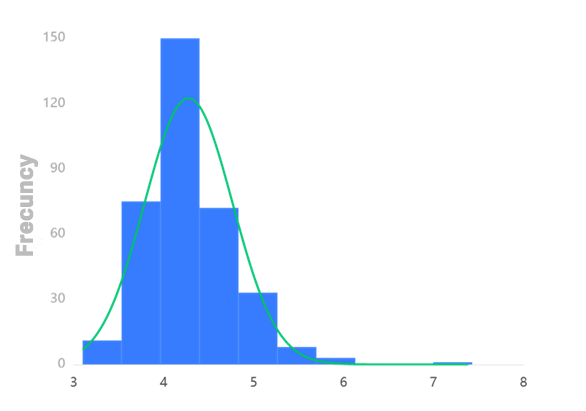
\includegraphics[width=\textwidth]{ATN_hist.png}
    \caption{Histogram of $ATN$}\label{subfig:ATN_hist}
    \end{subfigure}
    \begin{subfigure}[b]{.4\textwidth}
    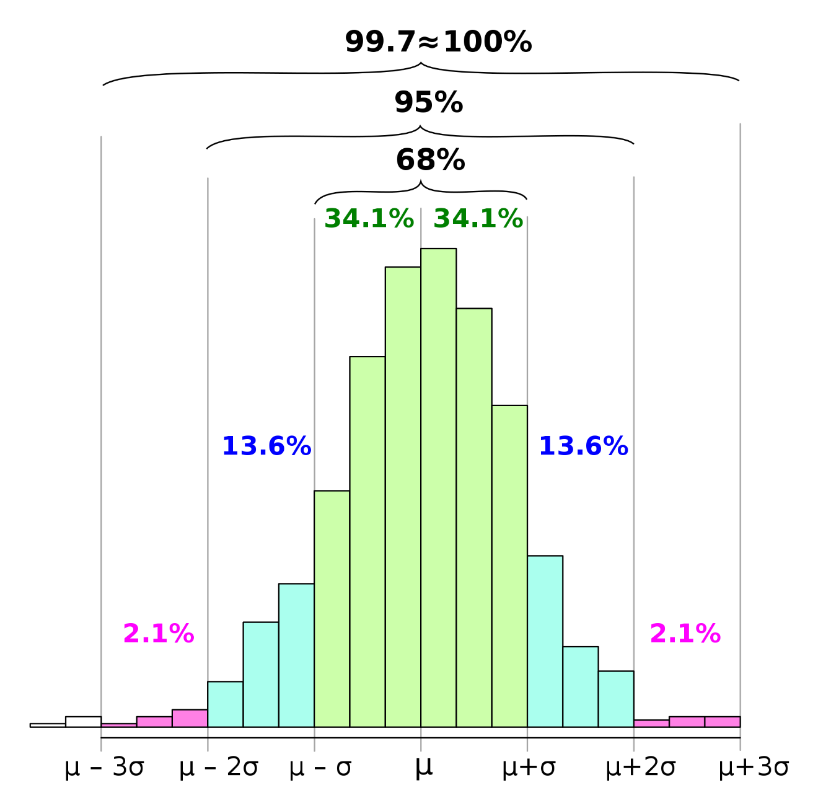
\includegraphics[width=\textwidth]{normal.png}
    \caption{Empirical Rule}\label{subfig:normal}
    \end{subfigure}
    \caption{}\label{fig:nd}
\end{figure}

\begin{figure}[htbp]
    \centering
    \begin{subfigure}[b]{.4\textwidth}
    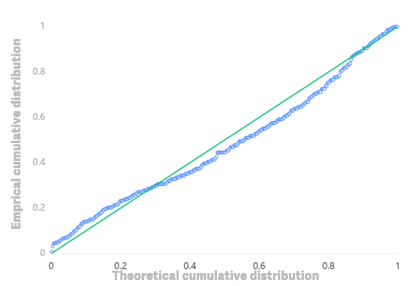
\includegraphics[width=\textwidth]{pp.png}
    \caption{P-P plot}\label{subfig:pp}
    \end{subfigure}
    \begin{subfigure}[b]{.4\textwidth}
    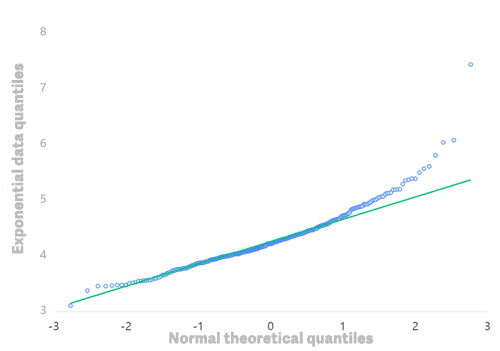
\includegraphics[width=\textwidth]{qq.png}
    \caption{Q-Q plot}\label{subfig:qq}
    \end{subfigure}
    \caption{Normality test P-P \& Q-Q plot}\label{fig:ppqq}
\end{figure}

The figure \ref{subfig:pp} shows the fit of the cumulative probability $P$ of the observation calculated by $ATN$ to the normal cumulative probability $P$. The higher the degree of fit, the more normal distribution.

The figure \ref{sub@subfig:qq} stands for "Quantile Quantile Plot". Test for normal distribution by comparing the probability distributions of different quantiles of the observed and predicted values (assuming normal distribution). The actual data is taken as the X-axis, and the quantile of the assumed normal data is taken as the Y-axis to make a scatter plot. The higher the coincidence degree between the scatter and the line, the more normal distribution is followed, and the larger the difference between the scatter points, the less normal distribution is followed.

In summary, the figure \ref{fig:ppqq} shows a better situation of you and sum, and the $ATN$ can be accepted as normal distribution.

\subsection{Measure of Difficulty}

The normal distribution is defined by two parameters: its mean $\mu$ and standard deviation $\sigma$. The mean determines the center of the distribution and the standard deviation determines the spread or width of the distribution.

According to the above normality test, we can conclude that the mean value $\mu = 4.277$ and the standard deviation $\sigma = 0.489$ for $ATN$. We divide $ATN$ into three intervals according to the empirical rule:

\begin{itemize}
    \item Easy: $ATN \in [\mu - \sigma, \mu - \sigma)$
    \item Normal: $ATN \in [\mu - \sigma, \mu + \sigma)$
    \item Hard: $ATN \in [\mu + \sigma, \mu + 3\sigma]$
\end{itemize}

68.27\% of the data of $ATN$ fall within $[\mu - \sigma, \mu + \sigma)$, we believe that the $ATN$ in this range reflects the middle difficulty of the word --- normal, and based on Wordle's mechanism, we believe that word difficulty is positively correlated with $ATN$. Since then, we are proud to announce our difficulty classification model:

% Python 代码示例
\begin{lstlisting}[language=Python, name={classification.py}]
    # Python3 code for difficulty classification
    if 4.277-3*0.489 <= ATN < 4.277-0.489:   tag = 'Easy'
    elif 4.277-0.489 <= ATN < 4.277+0.489:   tag = 'Normal'
    elif 4.277+0.489 <= ATN < 4.277+3*0.489: tag = 'Hard'
    else:                                    tag = 'error'
\end{lstlisting}


\subsection{Difficulty Prediction}
% TODO
Thanks to the work in MIMO XGBoost model, we can already predict with high accuracy the distribution of player tries (1 try-7 or more tries (X)) for a given word on a given day. Applying the formula \ref{eq:ATN}, we can get the $ATN$ for a given word, and the difficulty classification can be obtained from the model above.

Predict the difficulty classification of the word EERIE on 2023.03.01:
% TODO
\begin{enumerate}
    \item By using our feature extractor, we get the 13 attributes of EERIE.
    \item The 13 variables are used as input to the prediction model MIMO XGBoost to obtain the distribution of attempts for EERIE.
    \item Calculate the $ATN$ of EERIE according to formula \ref{eq:ATN} $ATN= (7.67\% \times 2 + 10.18\% \times 3 + 22.31\% \times 4 + 21.97\% \times 5 + 33.97\% \times 6 + 3\% \times 10) = 4.79$
    \item The difficulty classification of EERIE is obtained as hard according to the classification model.
\end{enumerate}


\subsection{Identify Important Attributes}
\begin{figure}
    \centering
    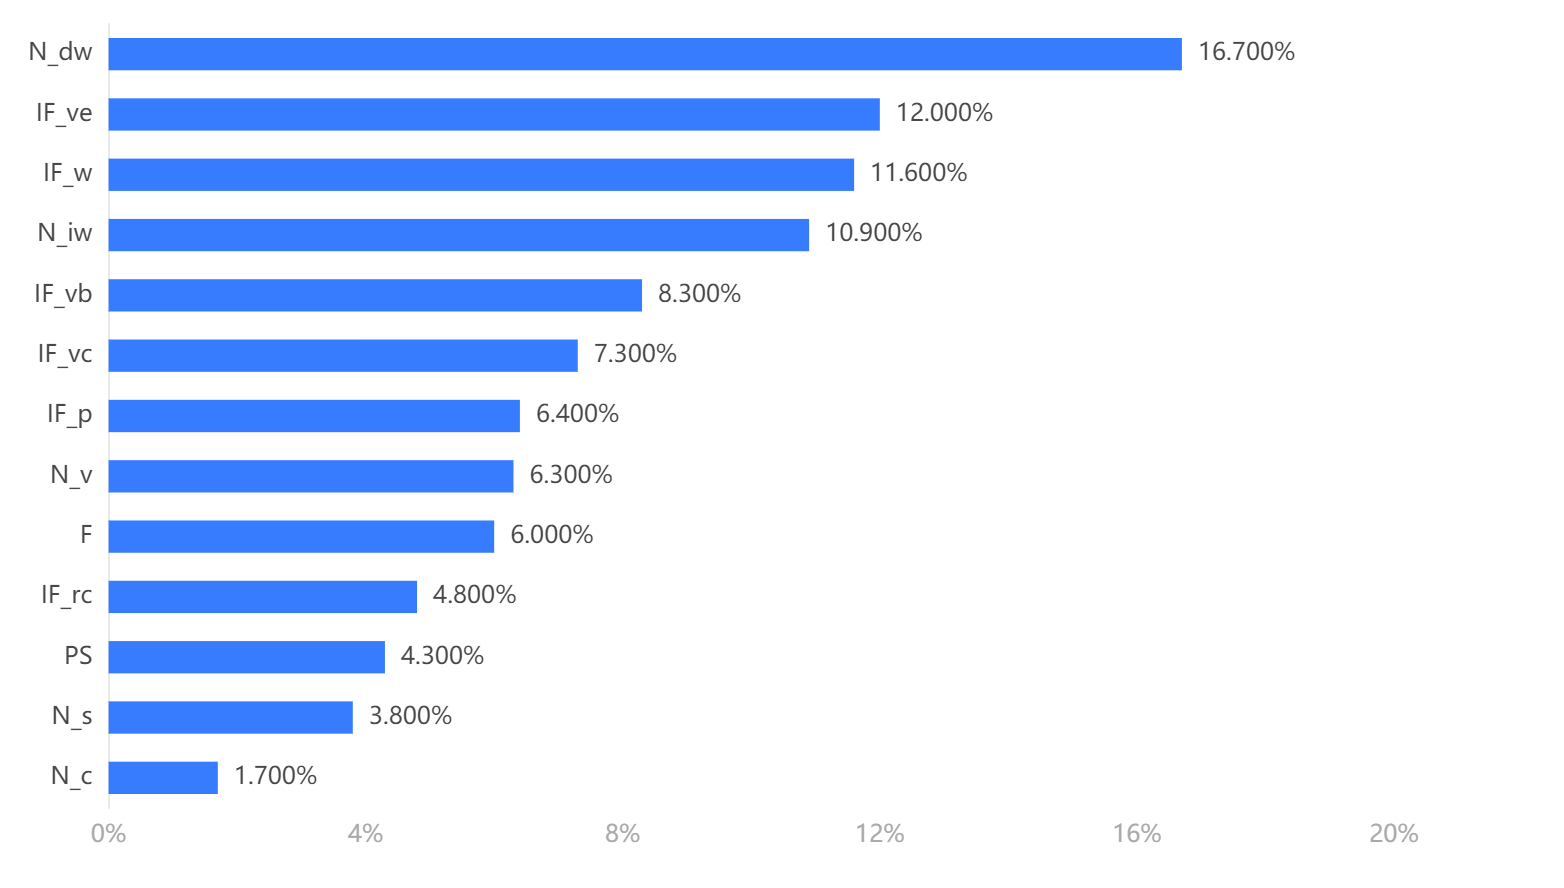
\includegraphics[width=.8\textwidth]{feature_percent.png}
    \caption{Importance of each attribute in classification}\label{fig:feature_percent}
\end{figure}
The upper bar chart generated from my model shows the proportion of importance of each attribute in the difficulty classification, where the number of duplicate words $N_{dw}$, vowel beginning or not $IF_{ve}$, workday or not $IF_w$ and the number of hours used alphabets $N_{iw}$ accounted for 16.7\% respectively, 12.0\%, 11.6\% and 10.9\%. This is in line with our general understanding, and also has a high compatibility with the Wordle recipes on social networking sites.

\subsection{Model Evaluation}
Since the classification model depends on the $ATN$ and the $ATN$ depends on the prediction model MIMO XGBoost. So the accuracy of classification model theoretically depends on MIMO XGBoost. Without further elaboration, please refer to the work in section 5.3.




% Q4之后
\section{Data Insights}


\begin{figure}[htbp]
\centering
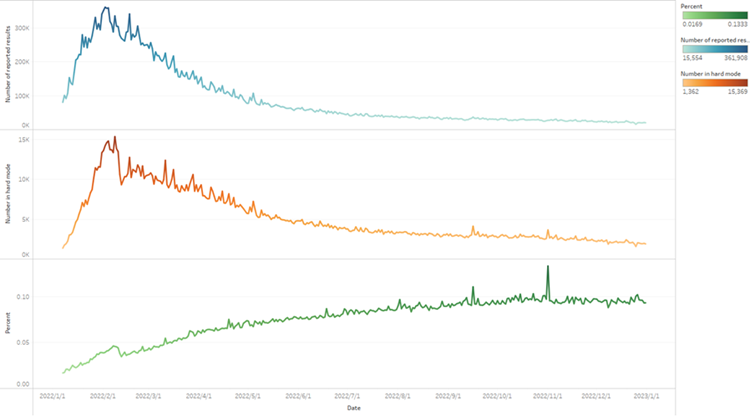
\includegraphics[width=.5\textwidth]{img/insight1.png}
\caption{Trends in three kinds of data}\label{fig:insight1}
\end{figure}
The above three graphs are the data graphs of the number of people who participate in the game, the number of people who choose the difficult mode, and the percentage of people who choose the difficult mode over time. From the figure, we can easily see that no matter what mode, the number of daily players first increases and then decreases, and the popularity of the game is lower than before. At the same time, we notice that the percentage of people in difficult mode is increasing slightly. Combined with the above two figures, we can roughly think that it is mainly caused by the decline of the total number of people, but this percentage also reflects that there are still a number of loyal users in difficult mode who are keen to challenge themselves in the word guessing game every day.

\begin{figure}[htbp]
\centering
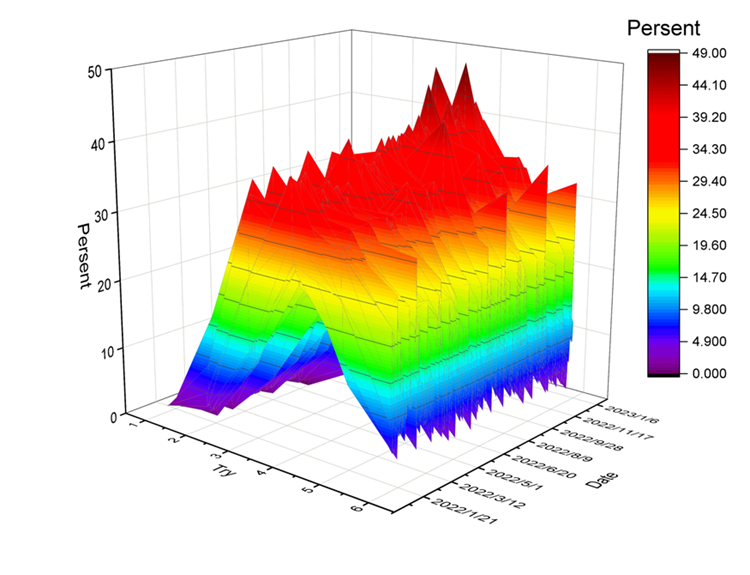
\includegraphics[width=.5\textwidth]{img/insight2.png}
\caption{The variation trend of different tyies under the time axis}\label{fig:insight1}
\end{figure}

The graph above shows the numerical relationship between the number of attempts, the date, and the percentage. When we look at the number of attempts on a given day, we can see that the distribution is roughly normal, with the daily high points of the percentage concentrated between 2, 3, 4, and 5 attempts, which confirms our conjecture about the distribution of the data. So the number of 1 and 7 attempts can be considered to be very low when excluding the exception of individual players, and this feature is in good agreement with our previous prediction for words.

\clearpage

\section{Sensitivity Analysis}

\begin{figure}[htbp]
\centering
\begin{subfigure}[b]{.4\textwidth}
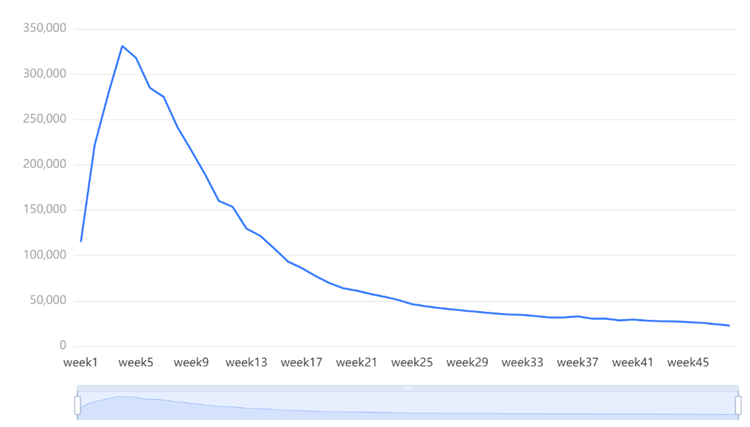
\includegraphics[width=\textwidth]{img/sensity1.png}
\end{subfigure}
\begin{subfigure}[b]{.4\textwidth}
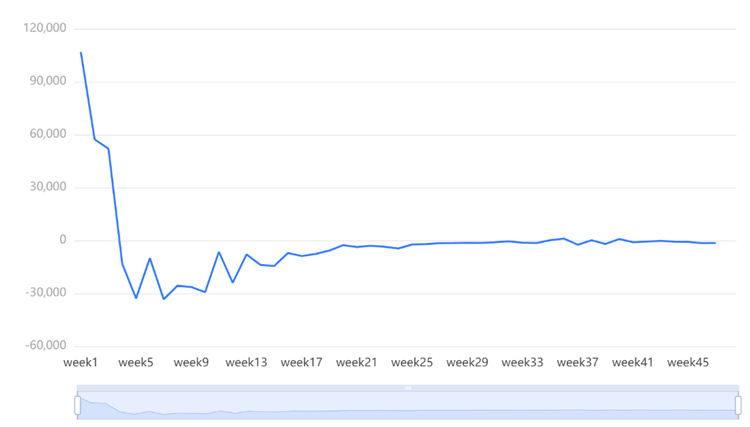
\includegraphics[width=\textwidth]{img/sensity2.png}
\end{subfigure}
\caption{Sensitivity analysis results of our two different order difference}\label{fig:subfigures}
\end{figure}

The above two graphs are the zeroth-order difference graph and the first-order difference graph in the ARIMA model. Although both of them perform well on the ADF test table, we can still see from the images that the first-order difference graph reflects a more stable time series, which is verified by our subsequent model data.

\section{Strengths and Weaknesses}
\subsection{Strengths}

\begin{itemize}
    \item Make the most of the information: when designing our measure, we considered other useful properties of the words in the provided data;
    \item Excellent model performance: Our high model fit and low error values indicate that our model performs well and that our measurements are accurate;
    \item Right method choice: We reveal a link between the number of no-tries, thanks to our choice of method;
    \item High robustness: In general, our model is not sensitive to changes in the values of the parameters.
\end{itemize}

\subsection{Weaknesses}
\begin{itemize}
    \item Some degree of randomness in feature extraction: we used random thinking when extracting some feature values;
    \item Limitations of the training word set: The word set we used to train in the XGboost model lacks scale to some extent, which may lead to biased prediction results;
 \end{itemize}



% 以下为信件/备忘录部分,不需要可自行去掉
% 如有需要可将整个 letter 环境移动到文章开头或中间
% 请在第二个花括号内填写标题,如「信件」(Letter)或「备忘录」(Memorandum)
\begin{letter}{Letter}
    \begin{flushleft}  % 左对齐环境,无首行缩进
    \textbf{To:} Puzzle Editor of the New York Times\\
    \textbf{From:} Team 2307004\\
    \textbf{Date:} February 20, 2023\\
    \end{flushleft}
    Dear Puzzle Editor of the New York Times, 
    
    Thank you very much for inviting us to conduct a data analysis of this interesting word-guessing game by Wordle. After understanding your specific requirements, we fully evaluated the feasibility of the task and are pleased to share our results with you.
    
    Firstly, after reading Wordle's rules in detail and processing and visualizing the data you provided, we extracted a set of attributes for the words, which we guessed would be an important measure of word difficulty through the extraction of word features. When analyzing the characteristics of the dataset we saw trends over time in data such as the number of players per day, which inspired us to use the Autoregressive Integrated Moving Average (ARIMA) model to fit the current player data and predict the interval of change in the number of players over time. We believe that we can achieve the same excellent results. Also, in response to your question about whether word attributes have an effect on difficulty mode selection rates, we have used Spearman's Correlation Analysis to make it clear that there is no significant correlation between the two.
    
    We then concluded that the average number of attempts (ATN) could be used to some extent as a characterization of word difficulty, and after performing the Shapiro-Wilk normality test, we used the Empirical Rule to classify words as easy, normal and hard, which also meant that the task of classifying word difficulty was transformed into a prediction task for ATN, which allowed us to use the above MIMO XGBoost Model again, further demonstrating the reasonableness and superiority of the model.
    
    Finally, in the course of our analysis we found that the number of Wordle players, in either mode, tends to rise and then fall in 2022, and in order to re-increase the flow of the game, we have summarized the following recommendations.
    \begin{itemize}
        \item Propose two words per day, one for difficult words and the other for easy or medium words, thus making the game a more friendly experience for both beginners and expert word-guessers.
        \item Hold regular special events on Wordle, such as holiday-related word-guessing games on special holidays.
        \item Add a social aspect to the current game mode, such as PK with friends, to make the game more interesting.
     \end{itemize}
    
    As we quote at the beginning of our paper, "The purpose of computation is insight, not numbers.", we offer more than just cold models and numbers, but through our analysis, we want to help Wordle re-engage players around the world and make word guessing more accessible to more people.
    
    Thanks for taking the time out of your busy schedule to read my letter. If you would like to know more about the results of the analysis, we would be glad to provide you with further assistance.
    \end{letter}
    
    
    % 参考文献,此处以 MLA 引用格式为例
    \begin{thebibliography}{99}
    \bibitem{1} Scientific Platform Serving for Statistics Professional 2021. SPSSPRO. (Version 1.0.11)[Online Application Software]. Retrieved from https://www.spsspro.com.
    \bibitem{2} Wang Yan. Application of time series analysis [M]. Beijing: China Renmin University Press 2005.
    \bibitem{3} Chen T , Guestrin C . XGBoost: A Scalable Tree Boosting System[J]. ACM, 2016.
    \bibitem{4} Xu Weichao. Review of Correlation Coefficients [J]. Journal of Guangdong University of Technology,2012,29(3):12-17.
    \bibitem{5} Ghatasheh, Nazeeh, Ismail Altaharwa, and Khaled Aldebei. "Modified Genetic Algorithm for Feature Selection and Hyper Parameter Optimization: Case of XGBoost in Spam Prediction." IEEE Access 10 (2022): 84365-84383.
    \bibitem{6} Yuan, Haitao, and Guoliang Li. “A Survey of Traffic Prediction: From Spatio-Temporal Data to Intelligent Transportation.” Data Science and Engineering, vol. 6, no. 1, Mar. 2021, pp. 63–85. Springer Link, https://doi.org/10.1007/s41019-020-00151-z.
    \bibitem{7} Wang, Y., \& Wang, Y. (2019). A survey of time series forecasting methods. Journal of Big Data, 6(1), 1-22.
    \bibitem{8} K. Kalpakis, D. Gada and V. Puttagunta, "Distance measures for effective clustering of ARIMA time-series," Proceedings 2001 IEEE International Conference on Data Mining, San Jose, CA, USA, 2001, pp. 273-280, doi: 10.1109/ICDM.2001.989529.
    \bibitem{9} S. Siami-Namini, N. Tavakoli and A. S. Namin, "The Performance of LSTM and BiLSTM in Forecasting Time Series," 2019 IEEE International Conference on Big Data (Big Data), Los Angeles, CA, USA, 2019, pp. 3285-3292, doi: 10.1109/BigData47090.2019.9005997.
    \bibitem{10} S. Siami-Namini, N. Tavakoli and A. Siami Namin, "A Comparison of ARIMA and LSTM in Forecasting Time Series," 2018 17th IEEE International Conference on Machine Learning and Applications (ICMLA), Orlando, FL, USA, 2018, pp. 1394-1401, doi: 10.1109/ICMLA.2018.00227.
    \bibitem{11} Y. Wang and Y. Guo, "Forecasting method of stock market volatility in time series data based on mixed model of ARIMA and XGBoost," in China Communications, vol. 17, no. 3, pp. 205-221, March 2020, doi: 10.23919/JCC.2020.03.017.
    \bibitem{12} C. Sheng and H. Yu, "An optimized prediction algorithm based on XGBoost," 2022 International Conference on Networking and Network Applications (NaNA), Urumqi, China, 2022, pp. 1-6, doi: 10.1109/NaNA56854.2022.00082.
    \bibitem{13} H. Zhu and A. Zhu, "Application Research of the XGBoost-SVM Combination Model in Quantitative Investment Strategy," 2022 8th International Conference on Systems and Informatics (ICSAI), Kunming, China, 2022, pp. 1-7, doi: 10.1109/ICSAI57119.2022.10005355.
    \end{thebibliography}

    % \bibliographystyle{IEEEtran}
    % \bibliography{references}{}
    \end{document}  % 结束

    
\section{Appendix B: Program Codes}
Here are the program codes we used in our research.

% 代码环境示例三则
% 如您的论文不需要展示代码,请删除
% 更多用法,请参考 listings 宏包文档

% Python 代码示例
\begin{lstlisting}[language=Python, name={test.py}]
# Python code example
for i in range(10):
    print('Hello, world!')
\end{lstlisting}

\end{subappendices}  % 附录内容结束

\end{document}  % 结束
